\documentclass[parskip=full]{scrartcl}

\usepackage[utf8]{inputenc} % use utf8 file encoding for TeX sources
\usepackage[T1]{fontenc} % avoid garbled Unicode text in pdf
\usepackage[german]{babel} % german hyphenation, quotes, etc
\usepackage{hyperref} % detailed hyperlink/pdf configuration
\usepackage{mathptmx} %Schriftart Times
\usepackage[scaled]{helvet} %
\usepackage{graphicx}
\hypersetup{ % ‘texdoc hyperref‘ for options
pdftitle={Pflichtenheft},
bookmarks=true,
}

\makeatletter
\setlength{\@fptop}{0pt}
\makeatother

\usepackage{csquotes} % provides \enquote{} macro for "quotes"
%TitlePage

{
\titlehead{\centering
\includegraphics[width=10cm]{Logo.png}}
\title{\fontsize{40}{48} \selectfont \textsc{Pflichtenheft}\\
{\fontsize{18}{18} \selectfont Multimediatool zum Testen von Videoencodern}}}
\author {Carina Weber, Jan Benedikt Schwarz, Johannes Werner, Noel Schuhmacher,\\
Sascha Rapp, Simon Grafenhorst}

\begin{document}
\maketitle
\thispagestyle{empty}
\newpage
\tableofcontents
\newpage
\section{Einleitung}
Vive (lang: Video veritatem) ist ein Programm zum Testen verschiedener Videoencoder. Man hat die Möglichkeit ein Video (mit Filtern und Artefakten) zu bearbeiten, welches dann von einem externen Encoder encodiert wird. Dieses encodierte Video kann dann wieder in Vive geladen werden. So kann komfortabel mit graphischen Visualisierungen entschieden werden, wie gut der Encoder das Video encodiert hat.
\newpage
\section{Zielbestimmung}
Vive ist ein Multimedia-Framework zum Vergleichen und zur Evaluation von Videoencodern.
\subsection{Musskriterien}
\subsubsection{Rohvideo auswählen und bearbeiten}
\begin{itemize}
\item Video laden
\item Aus einer Liste von Filtern mehrere Filter auswählen
\item Aus einer Liste von Artefakten mehrere Artefakte auswählen
\item Filter/Artefakte anpassen
\item Zuvor verwendete Konfigurationen (Filter/Artefakte) auswählen
\item Anzeigen einer Vorschau mit den angewandten Filtern/Artefakten
\item Video abspeichern
\end{itemize}
\subsubsection{Bewerten des Encoders}
\begin{itemize}
\item Das Rohvideo laden
\item Mehrere encodierte Videos laden
\item Bewertungskriterien berechnen
\item Unterschiede zwischen Roh- und encodiertem Video visualisieren
\item Bewertungskriterien/Videoeigenschaften/Metadaten visualisieren
\item Roh- und encodierte(s) Video(s) nebeneinander synchron abspielen
\end{itemize}
\newpage
\subsubsection{Sonstiges}
\begin{itemize}
\item Zustand des Programms als Projekt speichern
\item Projekt laden
\item Rückgängig/Wiederholen-Funktion
\item Das Programm hat eine GUI
\end{itemize}
\subsection{Wunschkriterien}
\begin{itemize}
\item Encoder integrieren
\item Manuelles Bewertungssystem
\item Pluginsystem für Filter und Artefakte
\item Sich bewegende Artefakte
\item Auswählen von Vorschau Frames
\item SSim. und VQuad-HD als objektive Bewertungskriterien
\end{itemize}
\subsection{Abgrenzungskriterien}
\begin{itemize}
\item Die Software ist ausschließlich in englischer Sprache verfügbar
\item Audio wird nicht beachtet
\item Korrektheit der Software wird gewährt bis zu einer Videauflösung von 1980x1020 Pixel
\item Das Programm akzeptiert ausschließlich Rohvideos im YUV Format und Videos in Formaten, die in der libavcodec Bibliothek enthalten sind.
\end{itemize}
\newpage
\section{Produkteinsatz}
Vive soll es Forschungseinrichtungen und Firmen ermöglichen Videoencoder einfach
miteinander zu vergleichen. So kann schnell ein optimaler Encoder für den jeweiligen Zweck
gefunden oder die Qualität eines vorhandenen geprüft werden. Aber auch Privatpersonen können
mit diesem Produkt die Funktionsweise eines Encoders kennenlernen oder einen Encoder für ein
Privatprojekt auswählen.
\subsection{Anwendungsbereiche}
\begin{itemize}
\item Forschungsprojekte
\item Kommerzielle Softwarentwicklung
\item Privatprojekte
\end{itemize}
\subsection{Zielgruppe}
\begin{itemize}
\item Forscher im Bereich Multimedia
\item Videoplattformbetreiber
\item Videobearbeiter
\item Privatanwender
\end{itemize}
\subsection{Betriebsbedingungen}
Die Betriebsbedingungen unterscheiden sich im Wesentlichen nicht zu denen normaler 
\linebreak
Software:
\begin{itemize}
\item Büroumgebung
\item Laufzeiten von bis zu 8h pro Tag sind zu erwarten
\end{itemize}
\newpage
\section{Produktumgebung}

\subsection{Hardware}
\begin{itemize}
\item AMD64 Prozessorarchitektur
\item Intel: Core i3 2100 oder neuer
\item AMD: Athlon II oder neuer
\item 5 GB freier Festplattenspeicher
\item Mindestens 4 GB Arbeitsspeicher
\item Monitorauflösung von mindestens 1240x1024
\end{itemize}
\subsection{Software}
\begin{itemize}
\item Linux 64 bit (getestet auf Ubuntu)
\item Qt Bibliothek Version 5.5.1
\item ffmpeg 2.7.2 oder höher
\item libavcodec
\end{itemize}
\newpage
\section{Funktionale Anforderungen}
\subsection{Musskriterien}
\subsubsection{Allgemein}
\textbf{/F0000/ Steuerlemente für Videos}

Videos können mit folgenden Steuerelementen angeschaut werden:
\begin{itemize}
\item Start/Pause-Button
\item Stop-Button
\item Timeline
\item Geschwindigkeitsauswahl:
\begin{itemize}
\item Frame by Frame
\item 0.25x
\item 0.5x
\item 0.75x
\item 1.0x
\item 1.25x
\item 1.5x
\item 1.75x
\item 2.0x
\end{itemize}
\end{itemize}

\textbf{/F0001/ Akzeptierte Rohdateitypen}

\begin{itemize}
\item YUV
\end{itemize}
\newpage
\textbf{/F0002/ Akzeptierte encodierte Dateitypen}
\begin{itemize}
\item Libavcodec kompatible Dateitypen
\end{itemize}

\textbf{/F0003/ Anzeigen von Aktionen in Statusleiste}

Folgende Aktionen werden in der Statusleiste angezeigt, falls sie aktiv sind:
\begin{itemize}
\item Anwenden von Filtern/Artefakten
\item Speichern des veränderten Videos
\item Laden der encodierten Videos (also Berechnung von PSNR,etc.)
\item Laden/Speichern von Projekten/Ergebnissen
\item Laden/Speichern von Filterkonfigurationen
\end{itemize}

\textbf{/F0004/ Rückgängig}

Es gibt eine globale Rückgängigfunktion.

\textbf{/F0005/ Wiederholen}

Es gibt eine globale Wiederholenfunktion.

\textbf{/F0006/ Projekt speichern}

Es können Projekte gespeichert werden.

\textbf{/F0007/ Projekt laden}

Das Projekt wird wieder geladen und die GUI auf den Stand des
Speicherns gesetzt. Wurden die gespeicherten Daten verändert kann die Korrektheit
des Programms nicht mehr garantiert werden. Fehlende Daten werden, wenn möglich, neu berechnet. 

\subsubsection{Rohvideo auswählen und bearbeiten}
\textbf{/F0100/ Auswahl mit Dateiauswaldialog}

Auswahl eines Videos mit einem Dateiauswahldialog. Erlaubte Dateitypen wie in /F0001/.

\textbf{/F0101/ Angabe von Eigenschaften}

Angabe von
\begin{itemize}
\item Auflösung
\item Pixelschema
\end{itemize}
um den in /F0001/ spezifizierten Dateityp korrekt einlesen zu können.

\textbf{/F0102/ Erlaubte Pixelschemata}

Für das in /F0101/ spezifizierte Pixelshema sind folgende Angaben erlaubt:
\begin{itemize}
\item 4:4:4
\item 4:2:2
\item 4:2:0
\item 4:1:1
\end{itemize}

\textbf{/F0103/ Auswahl kürzlich ausgewählter Videos}

Auswahl aus einer Liste mit den 10 zuletzt ausgewählten Videos. Angaben wie in /F0101/ müssen
nicht mehr gemacht werden.

\textbf{/F0104/ Auswahl von Filtern}

Auswahl von einem oder mehreren Filtern, die auf das Video gelegt werden.

\textbf{/F0105/ Filter: Kontrast}

Einstellbare Eigenschaften:
\begin{itemize}
\item Stärke
\end{itemize}

\textbf{/F0106/ Filter: Helligkeit}

Einstellbare Eigenschaften:
\begin{itemize}
\item Stärke
\end{itemize}
\newpage
\textbf{/F0107/ Filter: Sättigung}

Einstellbare Eigenschaften:
\begin{itemize}
\item Stärke
\end{itemize}
\textbf{/F0108/ Filter: Postereffekt}

Schränkt die Anzahl der Farben ein, aus denen das Video bestehen kann. Wenn diese Zahl höher ist als im Originalvideo, wird das Original nicht verändert.
Einstellbare Eigenschaften:
\begin{itemize}
\item Maximale Anzahl der Farben
\end{itemize}

\textbf{/F0109/ Filter: Blende}

Blendet das Video von einem schwarzen Bildschirm ein oder aus.
Einstellbare Eigenschaften:
\begin{itemize}
\item Ein-/Ausblende
\item Start-/Endframe
\end{itemize}

\textbf{/F0110/ Filter: Drehen}

Dreht das Video. Es ist dann permanent um die angegebene Gradzahl gedreht.
Einstellbare Eigenschaften:
\begin{itemize}
\item Grad der Drehung
\end{itemize}

\textbf{/F0111/ Filter: Rauschen}

Einstellbare Eigenschaften:
\begin{itemize}
\item Statisch/Zufällig/Muster
\item Stärke
\end{itemize}

\textbf{/F0112/ Filter: Negieren}

Berechnet das farbliche Negativ des Videos.

\textbf{/F0113/ Filter: Rand}

Fügt dem Video einen Rand hinzu, welcher es vergrößert. Von dem Video wird nichts abgeschnitten.
Einstellbare Eigenschaften:
\begin{itemize}
\item Oben/Unten/Rechts/Links
\item Dicke
\item Farbe
\end{itemize}

\textbf{/F0114/ Filter: Spiegeln}

Spiegelt das Video um eine Achse.
Einstellbare Eigenschaften:
\begin{itemize}
\item Horizontal/Vertikal
\end{itemize}

\textbf{/F0115/ Filter: Zoom}

Zoomt zum Mittelpunkt in das Video.
Einstellbare Eigenschaften:
\begin{itemize}
\item Stärke
\end{itemize}

\textbf{/F0116/ Filter: Skalieren}

Einstellbare Eigenschaften:
\begin{itemize}
\item Seitenverhältnis beibehalten
\item Auflösung/Verhältnis(z.B. 2 mal so groß)
\end{itemize}

\textbf{/F0117/ Filter: Schwarzweiß}

\textbf{/F0118/ Filter: Sepia}

\textbf{/F0119/ Filter: Vintage}

\textbf{/F0120/ Filter: Unschärfe}

Einstellbare Eigenschaften:
\begin{itemize}
\item Kanten beibehalten
\item Stärke
\end{itemize}

\textbf{/F0121/ Filter: Schärfe}

Einstellbare Eigenschaften:
\begin{itemize}
\item Stärke
\end{itemize}

\textbf{/F0122/ Filter: Farbbalance}

Verändere Intensität der Grundfarben.
Einstellbare Eigenschaften:
\begin{itemize}
\item Farbe
\item Stärke
\item Helle/Mittlere/Dunkle Pixel ändern
\end{itemize}

\textbf{/F0123/ Filter: RGB-Filter}

Filtert zwei der Farben heraus.
Einstellbare Eigenschaften:
\begin{itemize}
\item Farbe, die nicht gefiltert wird
\end{itemize}

\textbf{/F0124/ Filter: Kanten}

Zeichnet nur die Kanten.

\textbf{/F0125/ Auswahl von Artefakten}

Auswahl von einem oder mehreren Artefakten, die auf das Video gelegt werden.

\textbf{/F0126/ Artefakt: Gittermuster}

Einstellbare Eigenschaften:
\begin{itemize}
\item Anzahl der vertikalen und horizontalen Linien
\item Farbe
\item Dicke der Linien
\item Durchsichtigkeit
\end{itemize}

\textbf{/F0127/ Artefakt: Rechteck}

Zeichnet ein gefülltes Rechteck.
Einstellbare Eigenschaften:
\begin{itemize}
\item Farbe
\item Größe
\item Position
\item Durchsichtigkeit
\end{itemize}




\textbf{/F0128/ Anwendugsreihenfolge von Filtern/Artefakten}

Ein neu ausgewählter Filter/Artefakt wird an das Ende der Anwendungsreihenfolge angehängt.

\textbf{/F0129/ Ändern der Anwendungsreihenfolge}

Die Anwendungsreihenfolge der Filter/Artefakte kann beliebig geändert werden.

\textbf{/F0130/ Entfernen ausgewählter Filter/Artefakte}

Ausgewählte Filter/Artefakte können wieder entfernt werden.

\textbf{/F0131/ Abspeichern einer Filter/Artefakte Konfiguration}

Konfiguration von Filtern/Artefakten kann abgespeichert werden.

\textbf{/F0132/ Anzeigen einer Vorschau}

Die Vorschau des ausgewählten Videos mit den ausgewählten Filtern und Artefakten besteht aus zwei Stufen.

\textbf{/F0133/ 5 Frame Vorschau}

Wenn der Benutzer etwas an den Artefakten/Filtern ändert, werden 5 Frames aus dem Video sofort gerendert.

\textbf{/F0134/ Komplette Vorschau}

Nachdem der Nutzer auf einen entsprechenden Button geklickt hat, kann er das ausgewählte Video mit allen ausgewählten Filtern und Artefakten anschauen. Steuerelemente wie in /F0000/.

\textbf{/F0135/ Speichern des Videos}

Das veränderte Video kann abgespeichert werden. Das Dateiformat entspricht dem des Inputvideos. (Siehe /F0001/)
\newpage
\textbf{/F0136/ Laden einer Filter/Artefakte Konfiguration}

Gespeicherte Konfigurationen können wieder geladen werden.

\textbf{/F0137/ Alles zurücksetzen}

Ausgewählte Filter und Artefakte können alle auf einmal entfernt werden.
\subsubsection{Encodierte Videos bewerten}
\textbf{/F0200/ Encodierte Videos laden}

Laden von mehreren enodierten Videos. Die maximale Anzahl ist nicht beschränkt. Akzeptierte Dateitypen wie in /F0020/.

\textbf{/F0201/ Rohvideo laden}

Laden eines Rohvideos. Akzeptierte Dateitypen wie in /F0001/.

\textbf{/F0202/ Anzeigen der encodierten Videos}

Die geladenen Videos können angeschaut werden.

\textbf{/F0203/ Anzeigen des Rohvideos}

Das Rohvideo kann angeschaut werden.

\textbf{/F0204/ Steuerelemente}

Alle Videos aus /F0202/ und /F0203/ teilen sich einen Satz Steuerelemente. Steuerlemente wie in /F0000/.

\textbf{/F0205/ Anzeigen von Dateiattributen}

Folgende Attribute der Videodateien werden angezeigt:
\begin{itemize}
\item Dateiname
\item Dateigröße
\item Anzahl der verschiedenen Farben
\item Codec
\end{itemize}

\textbf{/F0206/ Anzeigen eines RGB-Histogramms}

Für jedes Video wird ein RGB-Histogramm angezeigt.

\textbf{/F0207/ Anzeigen eines PSNR-Graphen}

Für jedes encodierte Video wird ein PSNR-Graph angezeigt.

\textbf{/F0208/ PSNR-Graph als Timeline}

Durch klicken auf den PSNR-Graph wird zu der dazugehörigen Stelle im Video gesprungen. (Bei allen geladenen Videos wird zu dieser Stelle gesprungen).

\textbf{/F0209/ Farbunterschied zwischen Roh- und encodiertem Video anzeigen}

Anzeigen der Farbdifferenz der einzelnen Farbkanäle zwischen Roh- und encodiertem Video.

\textbf{/F0210/ Anzeigen von Makroblöcken}

Falls der Encoder Makroblöcke zum Komprimieren verwendet hat, können diese angezeigt werden.

\textbf{/F0211/ Speichern der Ergebnisse}

Die Ergebnisse der Analyse können gespeichert werden.

\textbf{/F0212/ Kommentar}

Zu jedem encodierten Video kann ein Kommentar geschrieben werden.
\subsection{Wunschkriterien}

\subsubsection{Encoder integrieren}
\textbf{/W0000/ Laden eines Encoders}

Der Encoder, der verwendet werden soll, kann mit einem Dateiauswahldialog ausgewählt werden.

\newpage
\textbf{/W0001/ Akzeptierte Dateitypen für Encoder}

Akzeptiert werden ELF32,ELF64 Dateien.

\textbf{/W0002/ Encoder interface}

Der Encoder muss über eine Konsole aufgerufen werden können mit dem Dateinamen zu dem zu encodierenden Video und verschiedenen Encodierungsmodi als Parameter.

\textbf{/W0003/ Spezifizieren von Parametern}

Man kann Parameter angeben, die dem Encoder übergeben werden.

\textbf{/W0004/ Parameterliste}

Mehrere verschiedene Parameter werden in einer Liste zusammengefasst.

\textbf{/W0005/ Mehrfaches aufrufen des Encoders}

Für jeden Eintrag in der Liste aus /F1210/ wird der Encoder aufgerufen.

\textbf{/W0006/ Gewährleistung}

Wenn der Encoder nicht korrekt arbeitet (z.B. nicht terminiert), kann die Korrektheit von Vive nicht garantiert werden.

\textbf{/W0007/ Laden der encodierten Videos}

Wenn alle encodierten Videos erzeugt wurden, werden sie automatisch geladen.

\subsubsection{Manuelles Bewertungssystem}
\textbf{/W0100/ Bewerten der encodierten Videos}

Die Qualität eines encodierten Videos kann mit einem 5-Sterne Bewertungssystem bewertet werden.

\textbf{/W0101/ Speichern der Bewertung}

Die Bewertung wird gespeichert.
\newpage
\textbf{/W0102/ Laden der Bewertung}

Beim Laden eines Projektes wird auch die 5-Sterne Bewertung geladen.


\subsubsection{Pluginsystem für Filter und Artefakte}

\textbf{/W0200/ Dynamisches Laden von Plugins}

Beim Programmstart werden Filter und Artefakte dynamisch geladen.

\subsubsection{Sich bewegende Artefakte}

\textbf{/W0300/ Bewegendes Rechteck}

Artefakte können sich nach vorgegebenen Mustern bewegen.

\subsubsection{Auswählen von Vorschau Frames}

\textbf{/W0400/ Vorschauframes}

Die in /F0133/ spezifizierte Vorschau wird so verändert, dass die Frames zur Vorschau selbst gewählt werden können und nicht fest vorgegeben sind.

\subsubsection{Weitere Bewertungskriterien}

\textbf{/W0400/ SSim}

SSim wird zusätzlich berechnet und angezeigt.

\textbf{/W0401/ VQuad-HD}

VQuad-HD wird zusätzlich berechnet und angezeigt.


\newpage
\section{Produktdaten}
\subsection{Musskriterien}
\textbf{/D001/ Filter/Artefakt Konfiguration abspeichern}

Abgespeichert wird:
\begin{itemize}
\item welche Filter/Artefakte ausgewählt wurden
\item die Reihenfolge, in der die Filter/Artefakte angewendet werden sollen
\item der jeweilige Zustand der einstellbaren Eigenschaften der Filter/Artefakte
\end{itemize}


\textbf{/D002/ Projekt speichern}

Gespeichert wird:
\begin{itemize}
\item Attribute aus /D003/
\item Absoluter Pfad zu den encodierten Videos
\item Absoluter Pfad zum Rohvideo
\item Zustand des ''Video and analysis'' - Tabs
\item Zustand des ''Filter and artifacts'' -Tabs
\end{itemize}

\textbf{/D003/ Ergebnisse speichern}

Gespeichert wird für jedes encodierte Video:
\begin{itemize}
\item PSNR-Graph
\item RGB-Histogramm
\item Farbdifferenz
\item Attribute aus /F0205/
\item Kommentar zum Video
\end{itemize}

\textbf{/D004/ Videos}

Mit Filtern und Artefakten veränderte Videos.

\subsection{Wunschkriterien}
\textbf{/D100/ 5-Sterne Bewertung}

Die Bewertung wird zusätzlich bei /D003/ mitgespeichert.

\textbf{/D101/ Zusätzliche Bewertungskriterien}

Die Bewertungskriterien werden zusätzlich zu /D003/ abespeichert.


\newpage
\section{Nichtfunktionale Anforderungen}
\textbf{/L01/ Reagierende Oberfläche}

Auch bei rechenintensiven Hintergrundaktionen reagiert das Programm auf Benutzereingaben.

\textbf{/L02/ Fehlerrobust}

Bei Fehlerhaften Videodateien oder Nutzereingaben soll das Programm nicht abstürzen.

\textbf{/L03/ Programmstart}

Das Programm soll zum Starten nicht mehr als 5 Sekunden benöntigen.

\textbf{/L04/ Filter/Artefakte anwenden}

Ein Filter soll im Schnitt für 300 Frames mit einer Auflösung von 176x144 nicht mehr als 2,5 Sekunden zum Berechnen benötigen.

\textbf{/L05/ PSNR oder RBG-Unterschied}

Das Berechnen des PSNR-Graphen oder der RGB-Unterschied soll nicht mehr als 5 Sekunden für 300 Frames mit einer Auflösung von 176x144 benötigen.

\textbf{/L06/ Laden eines Projektes}

Das Laden eines Projektes soll, sofern nichts neu berechnet werden muss, nicht mehr als 2 Sekunden benötigen.

\textbf{/L07/ Speichern eines Projektes}

Das Speichern eines Projektes soll, sofern alles bereits berechnet wurde, nicht mehr als 2 Sekunden benötigen.

\textbf{/L08/ Speichern einer Filterkonfiguration}

Das Speichern einer Filterkonfiguration soll nicht mehr als eine Sekunde benötigen.

\textbf{/L09/ Laden einer Filterkonfiguration}

Das Laden einer Filterkonfiguration soll nicht mehr als 0,5 Sekunden benötigen.

\newpage
\textbf{/L10/ Abspielen der Videos}

Die Videos sollen mit einer Verzögerung von maximal einer Sekunde auf Veränderungen der Steuerelemente reagieren.

\textbf{/L11/ Laden eines Rohvideos}

Das Laden eines Rohvideos soll nicht mehr als 2 Sekunden benötigen für ein Video mit 300 Frames und einer Auflösung von 176x144.

\textbf{/L12/ Laden eines encodierten Videos}

Das Laden eines encodierten Videos soll nicht mehr als 1 Sekunde benötigen.
\newpage
\section{Benutzungsoberflächer}
\subsection{Anforderungen}
Die Benutzungsoberfläche ist auf Mausbedienung ausgelegt, eine Bedienung ohne Maus muss dennoch möglich sein.
\begin{itemize}
\item DIN 66234, Teil 8 ist zu beachten
\item Die Benutzungsoberfläche wird aus Elementen des Qt Designer aufgebaut
\end{itemize}
\subsection{Beispieldesign}

\subsubsection{Videoauswahl}
\begin{figure}[htbp] 
\centering
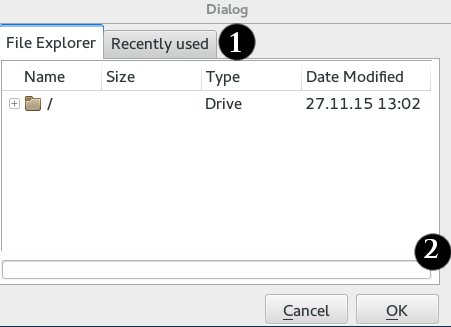
\includegraphics[width=0.7\textwidth]{ToViET/Screenshots/Fileselector.jpg}
\caption{Videoauswahl}
\begin{flushleft}
\item 1) Auswahl zwischen Dateiordnern und zuletzt benutzten Dateien
\item 2) Eingabebox 

\end{flushleft}
\end{figure}
\subsubsection{Auswahl der Rohvideo Eigenschaften}
\begin{figure}[htbp] 
\centering
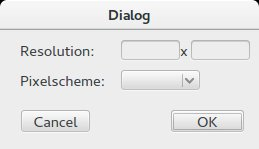
\includegraphics[width=0.5\textwidth]{ToViET/Screenshots/RawVidProperties.jpg}
\caption{Auswahl der Rohvideo Eigenschaften}

\end{figure}
\newpage
\subsubsection{Filter/Artefakte}
\begin{figure}[htbp] 
\centering
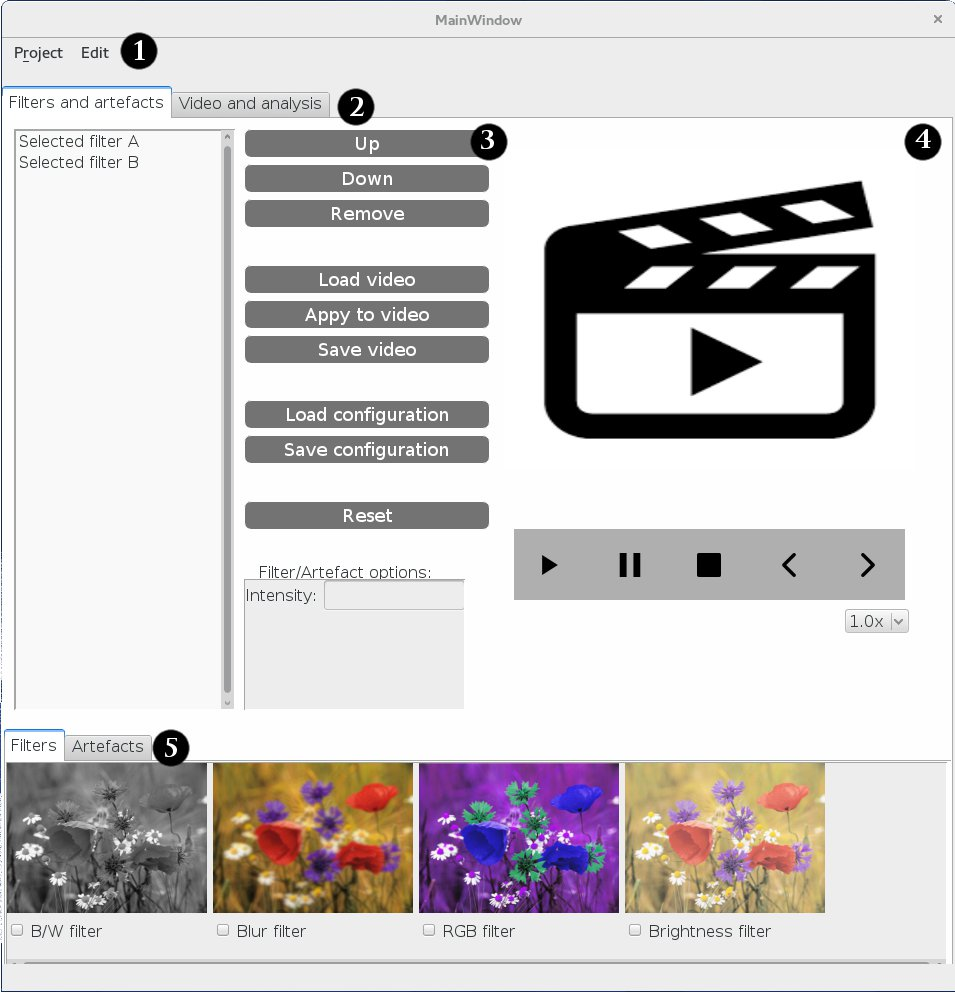
\includegraphics[width=0.7\textwidth]{ToViET/Screenshots/GUI_Filterselection.jpg}
\caption{Filter/Artefakte Auswahl}
\begin{flushleft}
\item 1) Auswahl zum Speichern,Öffnen und Bearbeiten des Projekts
\item 2) Wechsel zwischen Videobearbeitung und Analyse
\item 3) Auswahl für die Änderung von Filtern und Speichern des bearbeiteten Videos
\item 4) Vorschau der Filter in einzelnen Frames oder dem ausgewählten Video
\item 5) Auswahl von einsetzbaren Filtern und Artefakten
\end{flushleft}
\end{figure}
\newpage
\subsubsection{Wiedergabe und Auswertung}
\begin{figure}[htbp]
\centering
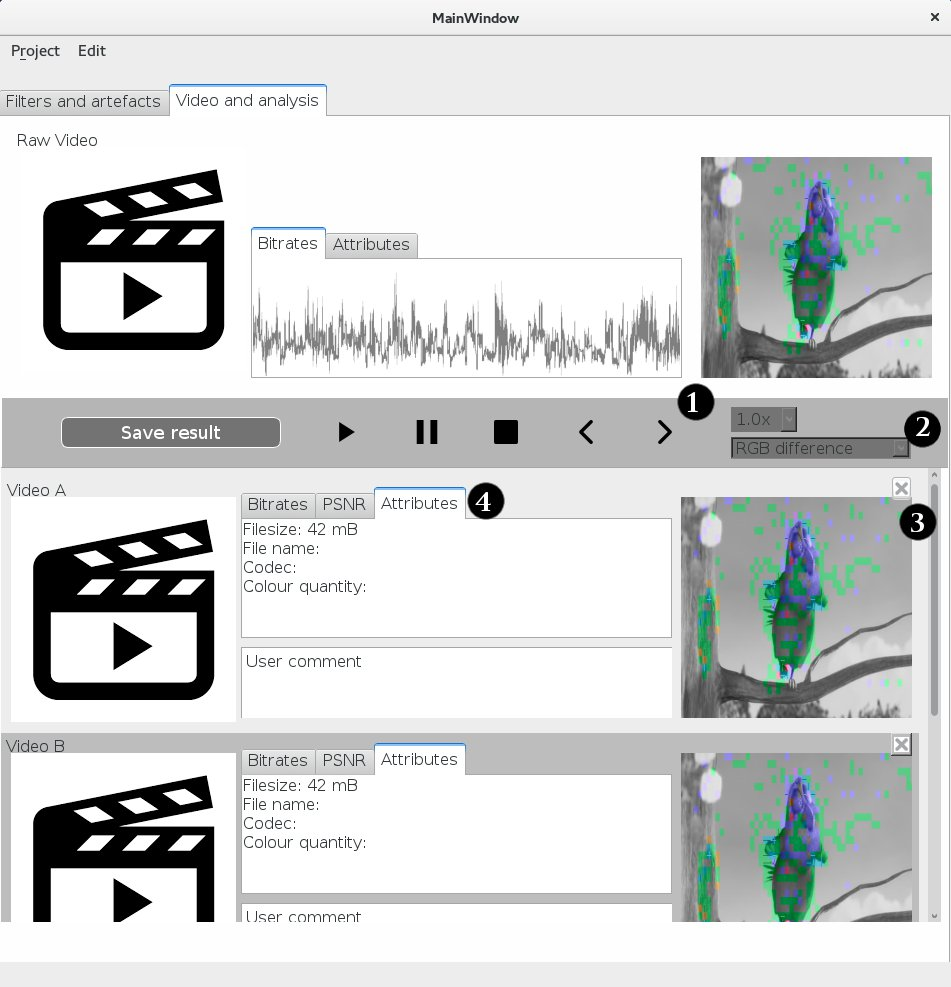
\includegraphics[width=0.75\textwidth]{ToViET/Screenshots/GUI_Videoanalysis}
\caption{Wiedergabe und Auswertung}
\begin{flushleft}
\item 1) Abspieloptionen des Videos
\item 2) Auswahl von Auswertungen einzelner Frames
\item 3) Auswertung einzelner Frames
\item 4) Auswertung von Videoeigenschaften 
\end{flushleft}
\end{figure}
\newpage
\section{Qualitätsbestimmungen}
\begin{tabular}{|c|c|c|c|c|}
\hline & Sehr wichtig & Wichtig & Weniger wichtig & Unwichtig \\
\hline Robustheit & • &  &  & \\ 
\hline Zuverlässigkeit & • &  &  & \\ 
\hline Korrektheit & • &  &  & \\ 
\hline Benutzerfreundlichkeit & • &  &  & \\ 
\hline Effizienz &  & • &  & \\ 
\hline Portierbarkeit &  &  & • & \\ 
\hline Kompatibilität &  &  & • & \\ 
\hline Modifizierbarkeit &  &  & • & \\ 
\hline Sicherheit &  &  &  & • \\ 
\hline 
\end{tabular} 
\newpage
\section{Systemmodelle}
\begin{figure}[htbp]
{\centering 
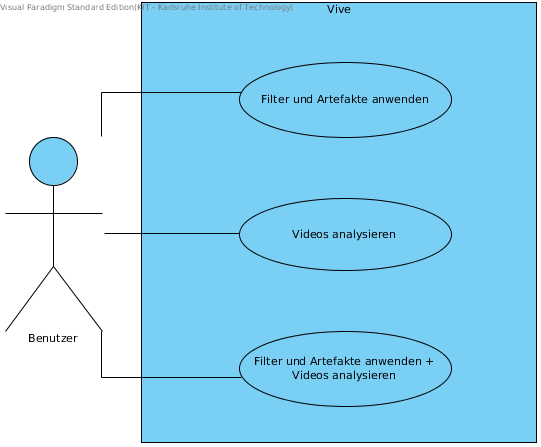
\includegraphics[width=0.7\textwidth]{UsecaseDiagrams/UseCaseDiagram1.png}
\caption{Komplettes Programm} }
\bigskip
Das Programm bietet zwei getrennte Funktionalitäten. Der Benutzer kann Filter und Artefakte auf eine Videosequenz anwenden und/oder mehrere Videos analysieren.

\end{figure}
\begin{figure}[htbp]
{\centering
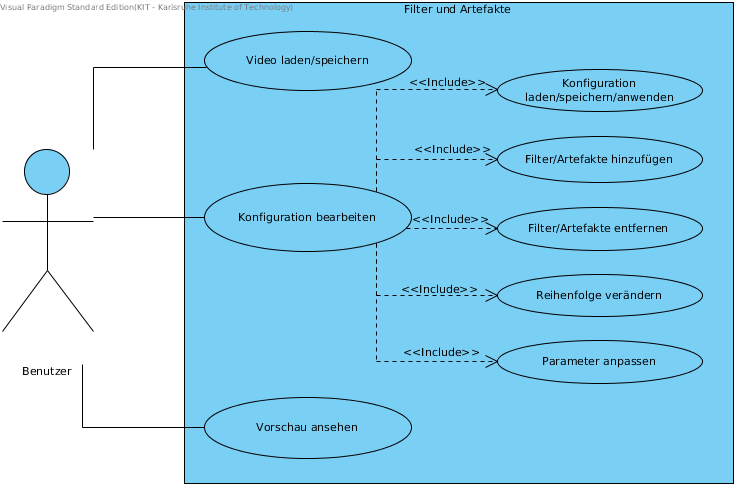
\includegraphics[width=0.7\textwidth]{UsecaseDiagrams/FilterundArtefakteanwenden.png}
\caption{Filter und Artefakte} }
\bigskip

Während des Anwendens der Filter und Artefakte hat der Benutzer die Möglichkeit ein Video zu laden/speichern, die aktuelle Konfiguration zu bearbeiten und sich eine Vorschau anzeigen zu lassen. 

Das Bearbeiten der Konfiguration beinhaltet das Laden/Speichern/Anwenden der aktuellen Konfiguration, das Hinzufügen/Entfernen von Filtern und Artefakten, sowie das Verändern ihrer Reihenfolge. Zudem können verschiedene Parameter jedes Filters und Artefakts angepasst werden.

\end{figure}
\begin{figure}[htbp]
{\centering
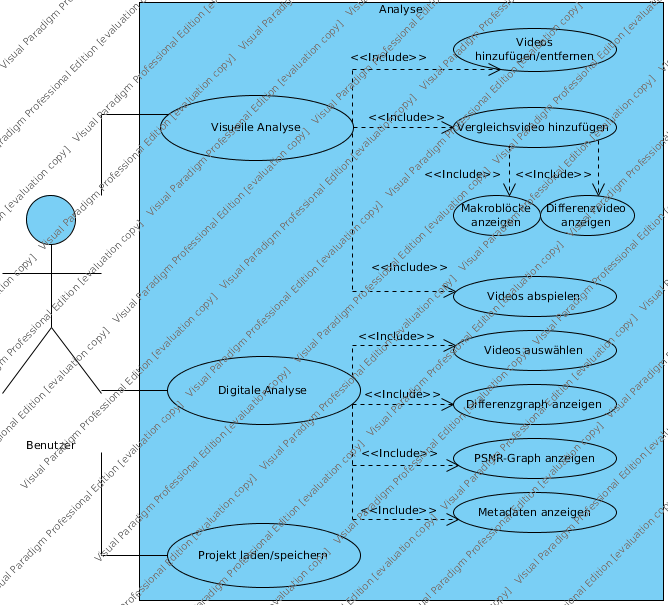
\includegraphics[width=0.7\textwidth]{UsecaseDiagrams/Analyse.png}
\caption{Videoanalyse} }
\bigskip
Der Benutzer hat die Möglichkeit mehrere Videos sowohl subjektiv als auch objektiv zu analysieren. 

Für die subjektive Analyse kann er Videos zur Übersicht hinzufügen, abspielen und wieder entfernen. Zudem kann er Differenzvideos hinzufügen oder Makroblocks ansehen.

Zur objektiven Analyse können PSNR-Graphen, Bitrate-Graphen und Differenzgraphen angezeigt werden.
Der Zustand des Projekts kann jederzeit gespeichert und geladen werden.

\end{figure}
\newpage
\section{Globale Testfälle und Szenarien}
\subsection{Testfälle}
Folgende Funktionssequenzen sind zu überprüfen:
\begin{itemize}
\item[]\textbf{/T000/}\qquad Oben auf "'Project"' und dann auf "'new"' klicken.
\item[]\textbf{/T001/}\qquad Zwischen den Reitern wechseln.
\item[]\textbf{/T002/}\qquad Oben auf "'Edit"' und dann auf "'undo"'/"'redo"' klicken.
\item[]\textbf{/T003/}\qquad Oben auf "'Project"' und dann auf "'Save"'/"'Save As"' klicken.
\item[]\textbf{/T004/}\qquad Oben auf "'Project"' und dann auf "'Load"' klicken.
\end{itemize}
\subsubsection{"'Filters and artefacts"' Reiter}
\begin{itemize}
\item[]\textbf{/T010/}\qquad "'Load video"' klicken und unter "'File Explorer"' ein Video auswählen.
\item[]\textbf{/T011/}\qquad "'Load video"' klicken und unter "'Recent used"' ein Video auswählen.
\item[]\textbf{/T012/}\qquad Filter auswählen und deren Reihenfolge und Intensität ändern.
\item[]\textbf{/T013/}\qquad Artefakte auswählen und deren Reihenfolge  ändern.
\item[]\textbf{/T014/}\qquad Filter/Artefakte auswählen und "'Apply to video"' klicken.
\item[]\textbf{/T015/}\qquad Filter/Artefakte auswählen und Vorschau des Videos testen.
\item[]\textbf{/T016/}\qquad Filter/Artefakte Auswahl durch klicken von "'Save configuration"' speichern.
\item[]\textbf{/T017/}\qquad Filter/Artefakte Auswahl durch klicken von "'Load configuration"' laden.
\item[]\textbf{/T018/}\qquad Filter/Artefakte auswählen und "'Save video"' klicken.
\item[]\textbf{/T019/}\qquad Aktuelle Filter/Artefakte Auswahl durch klicken von "'Reset"' löschen.
\end{itemize}
\subsubsection{"'Video and analysis"' Reiter}
\begin{itemize}
\item[]\textbf{/T020/}\qquad Auf das "'Add video"' klicken um ein Video hinzuzufügen.
\item[]\textbf{/T021/}\qquad Auf das "'x"' bei einem Video oben rechts klicken um ein Video zu entfernen.
\item[]\textbf{/T022/}\qquad Mehrere Videos durch "'Add video"' aufrufen.
\item[]\textbf{/T023/}\qquad Videos starten, pausieren und stoppen.
\item[]\textbf{/T024/}\qquad Videos mit verschiedenen Geschwindigkeiten abspielen.
\item[]\textbf{/T025/}\qquad Videos mit "'<"' und "'>"' und Frame für Frame  durchgehen.
\item[]\textbf{/T026/}\qquad Mit der Zeitleiste das Video durch springen.
\item[]\textbf{/T027/}\qquad Ergebnisse der Analyse betrachten.
\item[]\textbf{/T028/}\qquad Kommentar schreiben und auf "'Save result"' klicken.
\end{itemize}
\subsubsection{Fehlerfälle}
\begin{itemize}
\item[]\textbf{/T030/}\qquad Beschädigtes Projekt laden und Fehlermeldung "'Project could not be opened"' erhalten.
\item[]\textbf{/T031/}\qquad Beschädigtes Video Laden und Fehlermeldung "'Video could not be opened"' erhalten.
\item[]\textbf{/T031/}\qquad Falsches Dateiformat laden und die Fehlermeldung "'Invalid file format"' erhalten.
\end{itemize}
\subsection{Szenarien}
Folgende Szenarien sind zu überprüfen:
\begin{itemize}
\item[]\textbf{/T100/}\qquad Der Benutzer startet zunächst ein neues Projekt und fügt dann ein Rohvideo hinzu, indem er im "'Video and analysis"' Reiter auf "'Add video"' klickt. Daraufhin fügt er durch klicken von "'Add video"' eine encodierte Version des Videos hinzu. Danach betrachtet er die Videos zunächst mit 0.5x, 1.0x, 1.5x facher Geschwindigkeit und geht die Videos dann "'frame by frame"' durch. Nun betrachtet er den PSNR Graphen und die Makroblöcke sowie weitere Analyse Auswertungen. Zuletzt schreibt er einen Kommentar in das "'User comment"' Feld und speichert dann die Analyse durch klicken auf "'Save result"' und das Projekt durch klicken auf "'Save as"' oben unter "'Project"'.
\item[]\textbf{/T101/}\qquad Der Benuter startet ein neues Projekt. Dann lädt er im "'Filters and artefacts"' Reiter ein Video und wählt mehrere Filter/ Artefakte aus. Daraufhin verändert er die Reihenfolge der Filter/Artefakte und speichert das Video ab. Nachdem er das abgespeicherte Video encodiert hat fügt er dieses zusammen mit dem Rohvideo als neues Video im "'Video and analysis"' Reiter hinzu. Danach betrachtet er die Videos und die dazugehörigen Analyse Auswertungen. Zuletzt speichert er dies Ergebnisse mit einem Kommentar ab.
\item[]\textbf{/T102/}\qquad Der Benutzer lädt ein bereits existierendes Projekt durch klicken auf "'Project"' und "'Load"'. Er betrachtet zunächst die geladenen Videos und deren Analyse Auswertungen im "'Video and analysis"' Reiter. Daraufhin schaut er sich unter dem "'Filters and artefacts"' Reiter die ausgewählten Filter/Artefakte des zuletzt bearbeiteten Videos an. Danach schließt er das Programm.
\end{itemize}
\newpage
\section{Glossar}
\subsection*{5-Sterne Bewertungssystem}  
5 Sterne zur Bewertung, wobei 1 Stern die niedrigste Bewertung ist und 5 Sterne die höchste.

\subsection*{Artefakt} Eine Struktur, die über das Video gelegt wird, wie zum Beispiel ein Kreis oder eine Linie.
\subsection*{Benutzer} 
Weibliche oder männliche Person, die das Programm benutzt.
\subsection*{Encoder} 
Ein Programm zum komprimieren von Videodateien.
\subsection*{Filter} 
Ein Algorithmus, der Farbwerte nach einem bestimmten Muster verändert.
\subsection*{Frame}
Ein einziges Bild aus einem Video
\subsection*{Projekt} 
Ein Projekt beinhaltet die Pfade zu den geöffneten Videos sowie die eingestellten Filter und Artefakte.
\subsection*{PSNR-Graph} 
Ein Graph der auf der x-Achse Zeitwerte(Framenummer) enthält und auf der y-Achse den dazugehörigen PSNR-Wert.
\subsection*{PSNR-Wert} 
Peak signal-to-noise ratio ist ein Maß für das Verhältnis zwischen Signalrate und dem überlagerten Rauschsignal.
\subsection*{RGB-Histogramm} 
Ein Graph, der die Farbverteilung eines Videos anzeigt.
\end{document}
